% Created 2021-03-06 Sat 20:46
% Intended LaTeX compiler: xelatex
\documentclass[11pt]{article}
\usepackage{graphicx}
\usepackage{grffile}
\usepackage{longtable}
\usepackage{wrapfig}
\usepackage{rotating}
\usepackage[normalem]{ulem}
\usepackage{amsmath}
\usepackage{textcomp}
\usepackage{amssymb}
\usepackage{capt-of}
\usepackage{hyperref}
\usepackage{polyglossia}
\setotherlanguage{russian}
\usepackage{amsmath}
\usepackage{physics}
\setmainlanguage{russian}
\setotherlanguage{english}
\setmainfont{Times New Roman}
\usepackage{amsmath}
\usepackage{physics}
\usepackage{graphicx}
\usepackage{hyperref}
\author{Семен Синченко}
\date{\today}
\title{Гейты}
\hypersetup{
 pdfauthor={Семен Синченко},
 pdftitle={Гейты},
 pdfkeywords={},
 pdfsubject={},
 pdfcreator={Emacs 27.1 (Org mode 9.5)}, 
 pdflang={Russian}}
\begin{document}

\maketitle
\tableofcontents


\section{Описание лекции}
\label{sec:org05f72b6}
Из этой лекции мы узнаем:
\begin{itemize}
\item Какие есть основные однокубитные гейты
\item Как записывать многокубитные состояния
\item Какие есть многокубитные гейты
\item Конструирование многокубитных операторов
\end{itemize}

\section{Основные однокубитные гейты}
\label{sec:orgfffb5e1}
В прошлый раз мы познакомились с операторами Паули, а также гейтом Адамара. Теперь давайте посмотрим какие еще однокубитные гейты часто применяются в квантовых вычислениях и квантовом машинном обучнении.

\subsection{Гейты поворота вокруг оси}
\label{sec:orgfcbf212}
Повротные гейты играют центральную роль в квантовом машинном обучении. Вспомним на секунду, как выглядят наши однокубитные состояния на сфере Блоха:

\begin{center}
\begin{figure}[htbp]
\centering
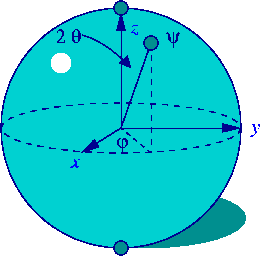
\includegraphics[width=0.35\textwidth]{./images/Blochcolor-alt.png}
\caption{Сфера Блоха}
\end{figure}
\end{center}

Гейты \(\hat{RX(\phi)}, \hat{RY(\phi)}, \hat{RZ(\phi)}\) осуществляют поворот на определенный угол \(\phi\) вокруг соответствующей оси на сфере Блоха.


Давайте внимательно рассмотрим это на примере гейта \(\hat{RY}\).



\subsubsection{Гейт \(\hat{RY}\)}
\label{sec:org37c5302}
Сам гейт определяется следующим образом:

\begin{align*}
\hat{RY(\phi)} = \begin{bmatrix}
\cos(\frac{\phi}{2}) & -\sin(\frac{\phi}{2}) \\
\sin(\frac{\phi}{2}) & \cos(\frac{\phi}{2})
\end{bmatrix}
\end{align*}

\begin{verbatim}
import numpy as np

def ry(state, phi):
    return np.array([
        [np.cos(phi / 2), -np.sin(phi / 2)],
        [np.sin(phi / 2), np.cos(phi /2)]
    ]) @ state
\end{verbatim}

Запишем наше состояние \(\ket{0}\)

\begin{verbatim}
basis = np.array([1 + 0j, 0 + 0j]).reshape((2, 1))
\end{verbatim}

Внимательно посмотрев на сферу Блоха, можно заметить, что повернув состояние из \(\ket{0}\) на \(\pi\) и измерив значение \(\hat{\sigma^z}\) мы получим 1, а повернув на \(-\pi\) 0:
\begin{verbatim}
def expval(state, op):
    return state.conj().T @ op @ state

pauli_x = np.array([[0 + 0j, 1 + 0j], [1 + 0j, 0 + 0j]])

np.allclose(expval(ry(basis, np.pi / 2), pauli_x), 1.0)
# True

np.allclose(expval(ry(basis, -np.pi / 2), pauli_x), -1.0)
# True
\end{verbatim}

Убедимся также, что вращение на угол, пропорциональный \(2\pi\) не меняет результата измерения. Возьмем случайное состояние:
\begin{align*}
\ket{\Psi} = \begin{bmatrix}
0.42 \\
\sqrt{1 - 0.42^2}
\end{bmatrix}
\end{align*}

\begin{verbatim}
random_state = np.array([0.42 + 0j, np.sqrt(1 - 0.42**2) + 0j]).reshape((2, 1))
\end{verbatim}

Измерим его по осям \(\mathbf{X}\) и \(\mathbf{Z}\), затем повернем его на угол \(2\pi\) и измерм снова:

\begin{verbatim}
pauli_z = np.array([[1 + 0j, 0 + 0j], [0 + 0j, 0j - 1]])

expval(random_state, pauli_z)
# array([[-0.6472+0.j]])
expval(random_state, pauli_x)
# array([[0.76232025+0.j]])

expval(ry(random_state, 2 * np.pi), pauli_z)
# array([[-0.6472+0.j]])
expval(ry(random_state, 2 * np.pi), pauli_x)
# array([[0.76232025+0.j]])
\end{verbatim}

\subsubsection{Другие гейты вращений}
\label{sec:org9ff96bc}
Аналогичным образом определяются гейты \(\hat{RX}\) и \(\hat{RZ}\):
\begin{align*}
\hat{RX(\phi)} = \begin{bmatrix}
\cos(\frac{\phi}{2}) & -i\sin(\frac{\phi}{2}) \\
-i\sin(\frac{\phi}{2}) & \cos(\frac{\phi}{2})
\end{bmatrix} \qquad \hat{RZ(\phi)} = \begin{bmatrix}
e^{-\frac{i\phi}{2}} & 0 \\
0 & e^{\frac{i\phi}{2}}
\end{bmatrix}
\end{align*}

В общем случае эти гейты могут быть также записаны следующим образом:
\begin{align*}
\hat{R^\sigma} = e^{-\frac{i\phi\sigma}{2}},
\end{align*}
где \(\sigma\) -- это один из операторов Пуали \(\sigma^x, \sigma^y, \sigma^Z\).

\subsection{Phase-shift гейт}
\label{sec:org487ca7a}
Другой важный гейт -- это так называемый phase-shift гейт, или \(\hat{U_1}\) гейт. Его матричная форма имеет следующий вид:
\begin{align*}
\hat{U_1(\phi)} = \begin{bmatrix}
1 & 0 \\
0 & y^{i\phi}
\end{bmatrix}
\end{align*}
\end{document}
